\stepcounter{slidesection}
\setbeamertemplate{background}[bgfirst]
\setbeamertemplate{footline}[first]
\subtitle{\theslidesection: Projektmanagement in der Softwareentwicklung}
\titlegraphic{Kapitel/ProjectManagement/Bilder/pmlogo.jpg}
\begin{frame}[noframenumbering]
\titlepage
\begin{textblock}{10}(4.75,15)
\cite{GesundheitssystemLogo}
\end{textblock}
\end{frame}
\setbeamertemplate{footline}[presentationbody] 
\setbeamertemplate{background}[bgbody]

\begin{frame}{Projektmanagement-Modelle}
    \begin{itemize}
		\item Viele Modelle sind in der Software-Entwicklung üblich:
		\begin{itemize}
			\item Waterfall
			\item V
			\item Rational Unified Process
			\item Iterative
			\item Spiral
		\end{itemize}
		\item<2-> Gruppenarbeit: 5 Gruppen, 15 Minuten Vorbereitung + maximal 3 Minuten Präsentation
		\item<3-> Motivation: 
		\only<3->{
			\begin{itemize} 
				\item In Startups überholt, aber in Industrie und Behörden noch immer Standard, also gut zu verstehen
				\item Langweilig, sich 5 Modelle anzuhören, also selber (besseres Verständnis, da eigene Auseinandersetzung)
			\end{itemize}
		}
	\end{itemize}
\end{frame}

\begin{frame}{ }
	\vspace{-0.2cm}
	\begin{figure}
		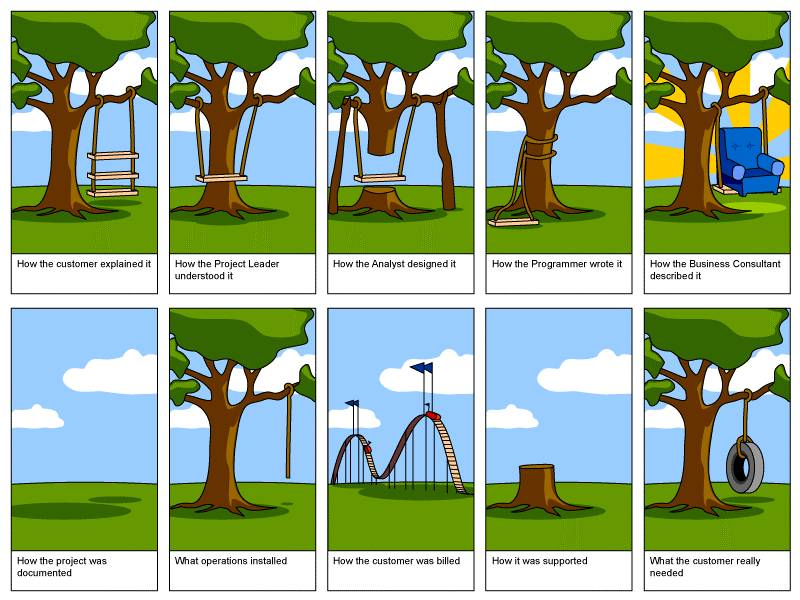
\includegraphics[height=0.85\textheight]{Kapitel/ProjectManagement/Bilder/pm.jpg}
		\caption{Projektmanagement im Alltag der Softwareentwicklung \cite{ProjectManagement}}
	\end{figure}
\end{frame}

\stepcounter{slidesection}
\setbeamertemplate{background}[bgfirst]
\setbeamertemplate{footline}[first]
\subtitle{\theslidesection: Agile Softwareentwicklung}
\titlegraphic{Kapitel/ProjectManagement/Bilder/pmlogo.jpg}
\begin{frame}[noframenumbering]
\titlepage
\begin{textblock}{10}(4.75,15)
\cite{GesundheitssystemLogo}
\end{textblock}
\end{frame}
\setbeamertemplate{footline}[presentationbody] 
\setbeamertemplate{background}[bgbody]

\begin{frame}{Agile}
	\begin{itemize}
		\item Erste Aufgabe des Projektmanagements: Team steuern, um zum Ziel zu kommen
		\item Nachteil: Abstand zu Code und Kunden (z.B. Merge-Manager)
		\item<2-> Industrie: PID (Proportional-Integrative-Derivative)-Controller
		\only<3->{
			\begin{itemize}
				\item Rausbekommen, wo man ist
				\item Kleinen Schritt in die Zielrichtung gehen
				\item Neugelerntes in Verständnis der aktuellen Lage einbauen
			\end{itemize}
		}
		\item<4-> Entscheidungen im agilen Kontext: Das tun, was zukünftige Anpassungen einfacher macht
	\end{itemize}
\end{frame}

\begin{frame}{Das Agile Manifest}
	\begin{itemize}
		\item 2001: Manifesto for Agile Software Development
		\item Kombination der Prinzipien von Extreme Programming, Pragmatic Programming, Scrum etc.
		\only<2-> {
			\item We value:
			\begin{itemize}
				\item \textbf{Individuals and interactions} over processes and tools
				\item \textbf{Working software} over comprehensive documentation
				\item \textbf{Customer collaboration} over contract negotiation
				\item \textbf{Responding to change} over following a plan
			\end{itemize}
		}
	\end{itemize}
\end{frame}

\begin{frame}{Agile ist tot!}
	DuckDuckGo: ``Agile certification'' - Industrie der Angst\\
	\only<2> {
		\begin{figure}
			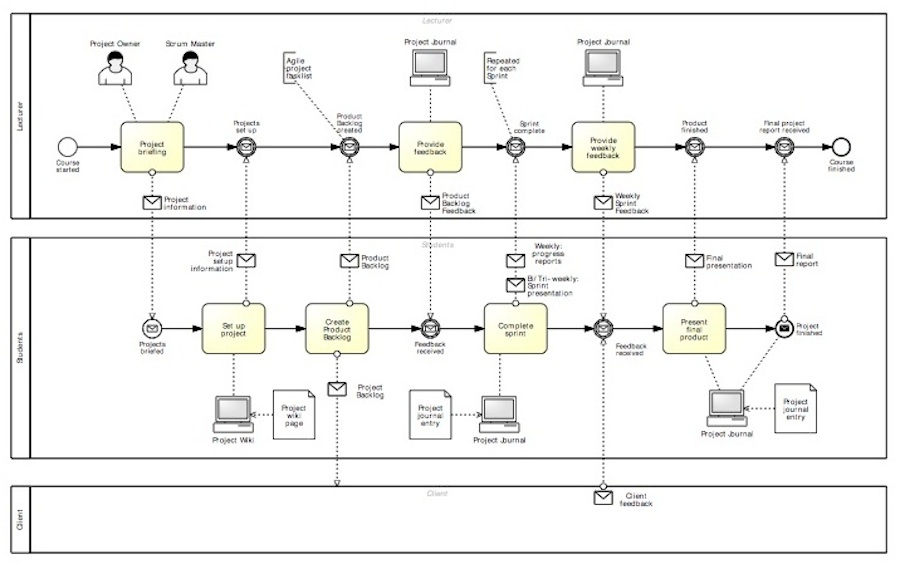
\includegraphics[height=0.58\textheight]{Kapitel/ProjectManagement/Bilder/AgileProcess.jpg}
			\caption{Prozessdokumentation für agiles Softwareprojekt \cite{AgileProcess}}
		\end{figure}
	}
	\only<3-> {
		\vspace{0.2cm}
		...Long live agile!
		\begin{itemize}
			\item ``Unsere Prozesse sind angelehnt an Scrum''
			\item ``Wir entwickeln zyklisch mit Hilfe eines Kanban-artigen Boards''
			\item ...
		\end{itemize}
	}
	\only<4->{Auflockerung vor nächstem Teil: Ballaufgabe}
	\only<5->{... Implikationen für die zweite Aufgabe des Projektmanagements: Team/Teams zu organisieren?}
\end{frame}

\begin{frame}{Prozessunterstützung}
	\begin{itemize}
		\item Scrum
		\only<1>{
			\begin{itemize}
				\item Sprint Planning
				\item Daily
				\item Increment
				\item Sprint Review
			\end{itemize}
		}
		\item<2-> User Stories
		\only<2> {
			\begin{itemize}
				\item Wer, was warum. Und: Was passiert sonst? Falls TDD/BDD: Case
				\item DOD, NFA
				\item Story Points (Planning Poker)
				\item Iterative Definition: Project Planning Board
				\item Mit Scrum: Burndown chart, velocity
			\end{itemize}
		}
		\item<3-> Kanban-Board(s)
		\item<4-> Verständnis vom Team-Prozess
		\only<4>{
			\begin{itemize}
				\item Forming
				\item Storming
				\item Norming
				\item Performing
				\item Adjourning
			\end{itemize}
		}
		\item<5-> Risiko-Management: Matrix, Lösungen
	\end{itemize}
\end{frame}



